\documentclass[11pt]{beamer}
\usetheme{Warsaw}
\usepackage[utf8]{inputenc}
\usepackage{amsmath}
\usepackage{amsfonts}
\usepackage{amssymb}
\author{Ritwik Sahani/ Aayush Goyal}
\title{The EM Algorithm}
%\setbeamercovered{transparent} 
%\setbeamertemplate{navigation symbols}{} 
%\logo{} 
%\institute{} 
%\date{} 
%\subject{} 
\institute{IIT Hyderabad}
\begin{document}


\begin{frame}
\titlepage{}
\end{frame}


\begin{frame}




\bigskip
\textsf{Suppose we have some data points x_{1}......x_{n}}
\begin{figure}
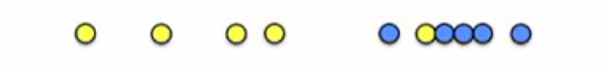
\includegraphics[scale=.3]{pic1.png}
\end{figure}
\textsf{and we also tell you that these points belong to two different probabilistic distributions, say, two gaussians such that we know which point belogs to which particular distribution.}\linebreak\linebreak
\textbf{Can we find the parameters $\mu_{b}, \sigma^{2}$ for the two gaussians?}\linebreak\linebreak

\textbf{Indeed, we can.}\linebreak\linebreak
\textsf{$\mu = \sum_{i=1}^{n_{b}}\frac{x_{i}}{n_{b}}$}\linebreak
\textsf{$\sigma^{2} = \sum_{i=1}^{n_{b}}\frac{(x_{i} - \mu_{b})^{2}}{n_{b}}$\linebreak
and similarly for the other distribution.}

\end{frame}



\begin{frame}



\textsf{Now, suppose data points are there but we don't know the as to which gaussian  a particular point belongs.}
\begin{figure}
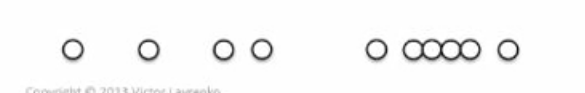
\includegraphics[scale=.3]{pic3.png}
\end{figure}
\textsf{But what we do know is that these come from two gaussians, whose parameters $\mu, \sigma^{2}$ is known}\linebreak\linebreak
\textbf{Can we, for each point, decide which of the two gaussians it is more likely to belong to?}\linebreak
\textsf{Yes, this can be done by claculating a posteriori prob.}\linebreak\linebreak
\textsf{$P(b|x_{i}) =\frac{ P(x_{i}|b)P(b)}{P(x_{i}|b)P(b) + P(x_{i}|a)P(a)}$}\linebreak
\textsf{where $P(x_{i}|b)$ can be obtained from the gaussian $N(\mu_{b}, \sigma_{b}^{2})$}
\end{frame}


\begin{frame}
\begin{figure}
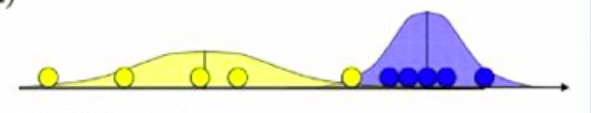
\includegraphics[scale=.3]{pic2.png}
\end{figure}
\textbf{But what happens, if we neither knew the source gaussian, nor their parameters?}\linebreak\linebreak
\textsf{Then we use the EM algorithm method, an iterative method, to find the same.}
\end{frame}


\begin{frame}
\textbf{Step-1: Expectation}\linebreak
\linebreak
\textsf{Creates a function for the expectation of the log-likelihood evaluated using the
current estimate for the parameters.}\linebreak
$\star$
\textbf{ Basically we will assume some initial parameters and assign each point with its a- posteriori probability}
\linebreak
\linebreak
\linebreak
\linebreak\linebreak
\textbf{Step-2: Maximization}
\linebreak

\textsf{Which computes parameters maximizing the expected log-likelihood found on the
E step. These parameter-estimates are then used to determine the distribution of
the latent variables in the next E step.}\linebreak
$\star$
\textbf{ Basically, we will again calculate the parameters for the next E -step }

\end{frame}


\begin{frame}
\textbf{Introduction}
\linebreak\linebreak
\textsf{The EM algorithm is used to find (local) maximum likelihood parameters of a
statistical model in cases where the equations cannot be solved directly. Typically
these models involve latent variables in addition to unknown parameters and known
data observations. That is, either missing values exist among the data, or the model
can be formulated more simply by assuming the existence of further unobserved
data points. For example, a mixture model can be described more simply by
assuming that each observed data point has a corresponding unobserved data
point, or latent variable, specifying the mixture component to which each data point
belongs.}
\end{frame}


\begin{frame}
\textbf{Two-Component Mixture Model}\linebreak
\textsf{We consider a simple mixture model for density estimation,
and the corresponding EM algorithm for carrying out maximum likelihood
estimation.}



\begin{figure}
\begin{flushleft}
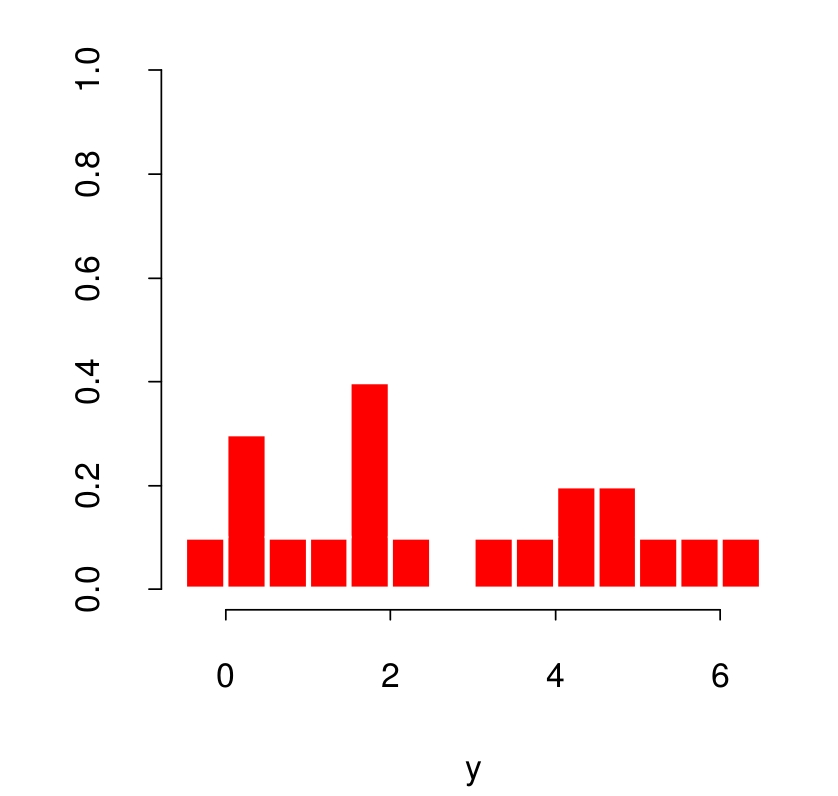
\includegraphics[scale=0.2]{fig1.jpg}
\label{Histogram of data}
\end{flushleft}



\begin{flushright}
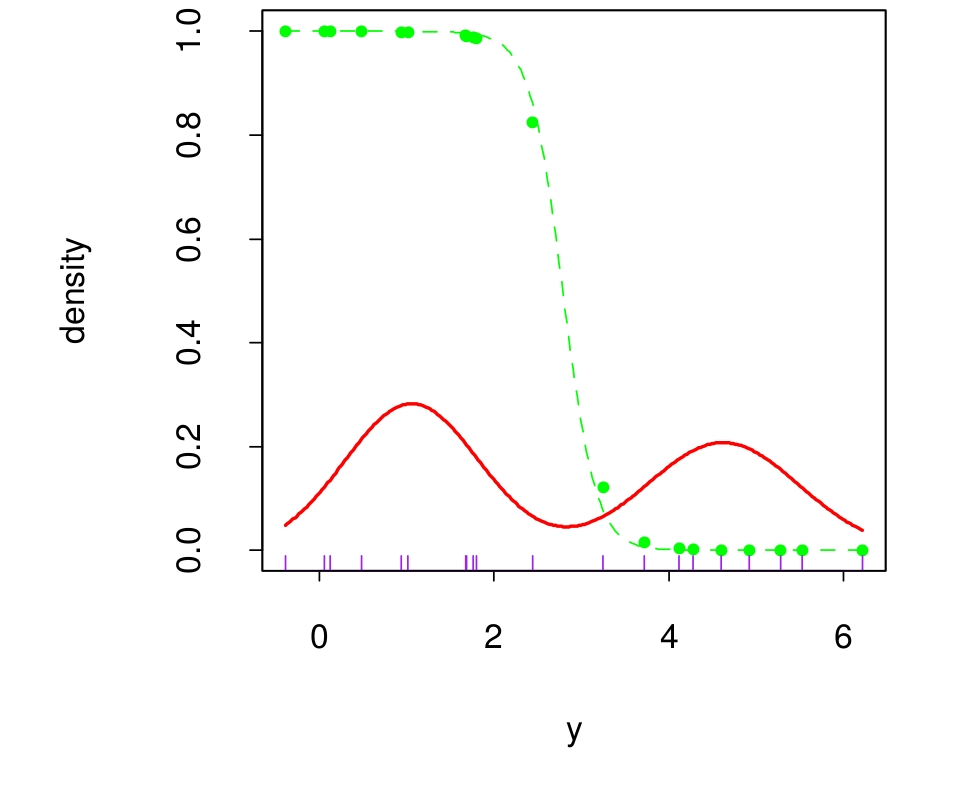
\includegraphics[scale=0.2]{fig2.jpg}
\label{Maximum likelihood fit
of Gaussian densities (solid red) and
responsibility (dotte green) of the left
component density for observation y,
as a function of y}
\end{flushright}
\end{figure}

\end{frame}


\begin{frame}
\begin{figure}
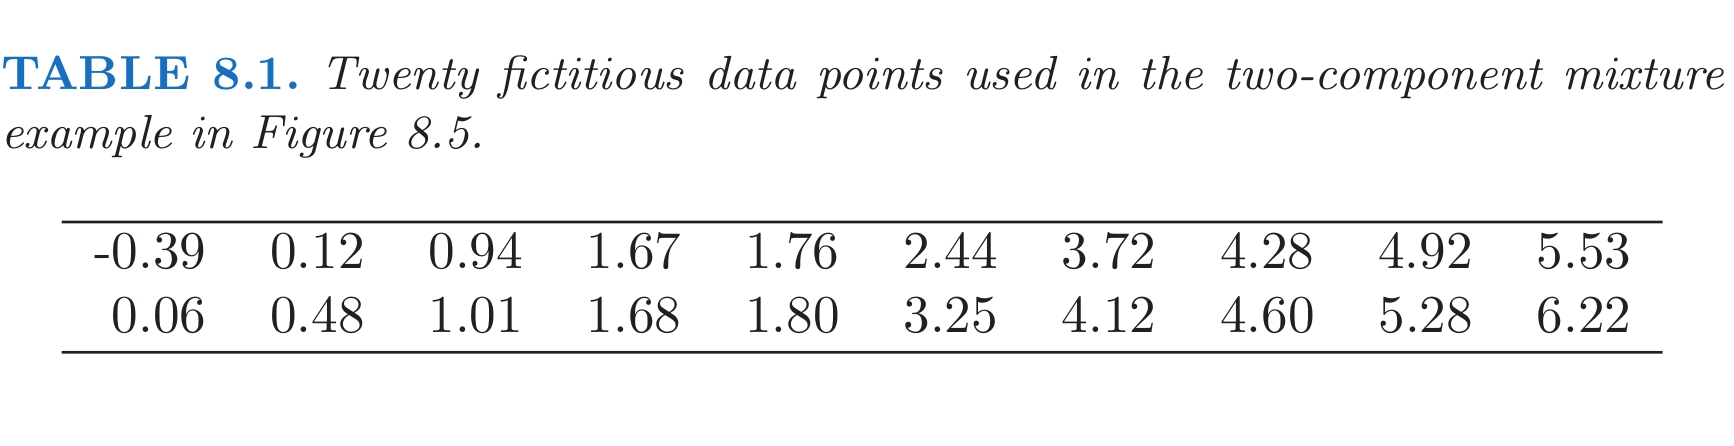
\includegraphics[scale=0.15]{fig3.jpg}
\end{figure}
\textsf{Due to Bimodalty of data Gaussian distribution would be inappropriate. So we
will model Y as a mixture of two distinct distributions.\linebreak\linebreak
$Y_{1} \equiv N(\mu_{1},  \sigma_{12}) $\linebreak
$Y_{2} \equiv N(\mu_{2},  \sigma_{22}) $\linebreak
$Y &= (1-\Delta)*Y_{1} + \Delta * Y_{2} $\linebreak
where $\Delta \in \{0, 1\}$ with $Pr(\Delta &= 1) = \pi $\linebreak\linebreak
This generative representation is explicit: generate a $\Delta \in \{0, 1\} $ with
probability $\pi$, and then depending on the outcome, deliver either Y_{1}  or  Y_{2} .
Let $\phi$ $\theta$ (x) denote the normal density with parameters $\theta = (\mu, \sigma_{2} )$. Then the
density of Y is\linebreak
$gY(y) = (1- \pi)\phi \theta_{1} (y)  + \pi\phi \theta_{2} (y).$}

\end{frame}


\begin{frame}
\textsf{Now suppose we wish to fit this model to the data in Figure 8.5 by maximum likelihood.The parameters are\linebreak
$\theta = (\pi, \theta_{1} , \theta_{2}) = (\pi, \mu_{1} , \sigma_{12} , \mu_{2} , \sigma_{22})$\linebreak
The log-likelihood based on the N training cases is}\linebreak\linebreak
$l(\theta; Z) = \sum_{i=1}^{N}  log[(1- \pi)\phi \theta_{1} (y_{i}) + \pi\phi \theta_{2} (y_{i} )]$\linebreak\linebreak
\textsf{Direct maximization of $l(\theta; Z)$ is quite difficult numerically, because of
the sum of terms inside the logarithm. There is, however, a simpler approach. We consider unobserved latent variables $\theta_{i}$ taking values 0 or 1 as
in (8.36): if $\Delta_{i} = 1 $then $Y_{1}$ comes from model 2, otherwise it comes from
model 1.\linebreak\linebreak
$l_{0}(\theta;Z,\Delta) = \sum_{i=1}^{N}[(1-\Delta_{i})log\phi_{\theta_{1}}(y_{i}) + \Delta_{i}log\phi_{\theta_{2}}(y_{i})] + \sum_{i=1}^{N}[(1-\Delta_{i})log(1-\pi)(y_{i}) + \Delta_{i}log\pi]$}
\end{frame}


\begin{frame}

\textsf{\linebreak\linebreak
Now we apply the E-M Algorithm for Two-component Gaussian mixture}
\begin{figure}
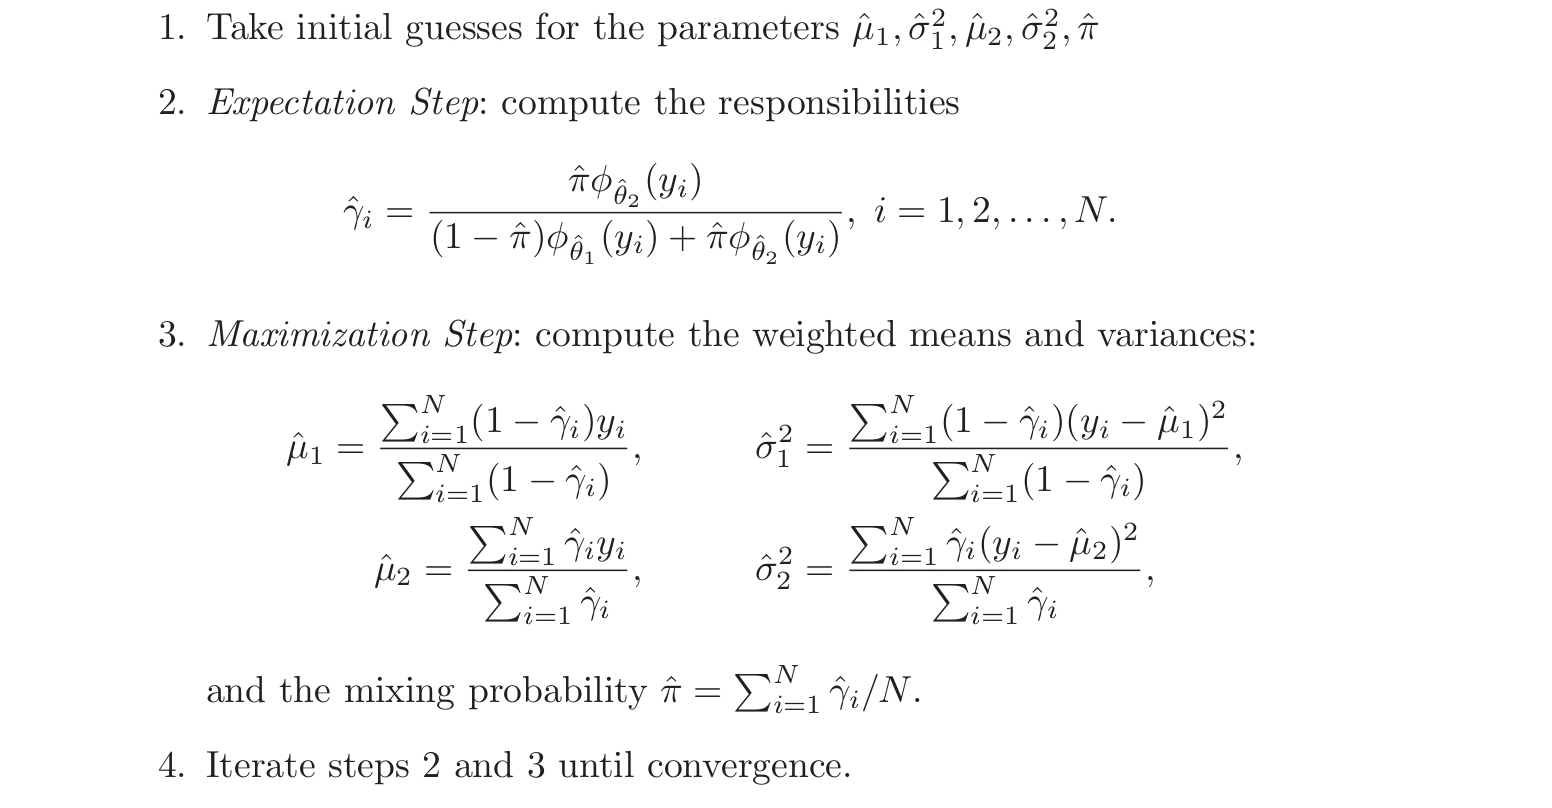
\includegraphics[scale=.315]{fig10.jpg}
\end{figure}
\end{frame}







\end{document}
